\subsection{Gnomonische Projektion}
\label{sec:gnomic}
In der gnomonischen Projektion werden alle Längenkreise als gerade Linien dargestellt.
Das Besondere der gnomonischen Projektion ist das der Projektionspunkt im Mittelpunkt der Erde liegt.
Da hier von Innen nach Außen projiziert wird, nimmt die Verzerrung mit der Entfernung vom Kartenmittelpunkt zu. Die gnomonische Projektion ist keine globale Projektion.\\

\begin{figure}[hbtp]
\centering
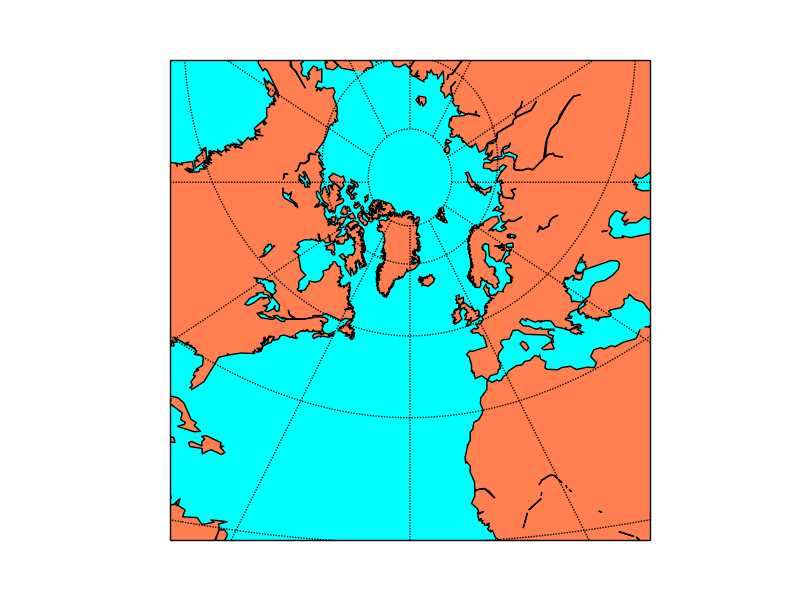
\includegraphics[scale=0.5,origin=c]{/Users/student/seminar/Kartendarstellungen/seminar/gnom} \caption{Gnomonische Projektion}
\end{figure}
\newpage 